\documentclass{beamer}

\usepackage{comment}
\usepackage{tabularx}
\usepackage{bm}
\usepackage{amsmath}
\usepackage{amssymb}
\usepackage{amsthm}
\usepackage{mathtools}


\def\imagetop#1{\vtop{\null\hbox{#1}}}

\def \lecturetitle {A coordinate gradient descent method for nonsmooth separable
  minimization}
\def \slidestring {\insertframenumber}

\setbeamercolor{alerted text}{fg=gray}
\author{Paul Tseng and Sangwoon Yun, 2009 \\ Presented by Matt Wytock \\ MLD Journal Club}
\usepackage{hyperref}
\usepackage{amsmath}
\usepackage{amssymb}
\usepackage{fancybox}
\usepackage{fancyvrb}
\usepackage{xcolor}
\usepackage{amsthm}
\usepackage{graphicx}
\usepackage{multirow}
\usepackage{gensymb}

%\usepackage{tcolorbox}


\definecolor{lightblue}{rgb}{.161,.502,.725}

\setbeamercolor{normal text}{fg=white,bg=black}
\setbeamercolor{item}{parent={local}}
\setbeamercolor{alerted text}{fg=red}

\setbeamercolor{title}{fg=lightblue}
\setbeamercolor{frametitle}{fg=lightblue}

\usefonttheme[onlymath]{serif}

\setbeamertemplate{navigation symbols}{}
\setbeamertemplate{frametitle}
{
\begin{centering}
\vspace{15pt}
\textbf{\insertframetitle}\par
\end{centering}
}

%\setbeamertemplate{footline}{\hspace{15pt}\tiny{\classnumber: \lecturetitle
%\hfill\insertframenumber}\hspace{15pt} \vspace{15pt}}
%\setbeamertemplate{footline}{\hfill \slidestring\hspace{10pt}\vspace{10pt}}
\setbeamertemplate{}



% small centered block
\newenvironment<>{varblock}[2][\textwidth]{
    \begin{center}
      \begin{minipage}{#1}
      \renewcommand{\'}{\symbol{13}}
        \setlength{\textwidth}{#1}
        \setlength{\leftmargin}{12pt}
          \begin{actionenv}#3
            \def\insertblocktitle{#2}
            \par
            \usebeamertemplate{block begin}
            \begin{semiverbatim}}
  {\par \end{semiverbatim}
      \usebeamertemplate{block end}
    \end{actionenv}
  \end{minipage}
\end{center}}


% itemize seperation
\newlength{\wideitemsep}
\setlength{\wideitemsep}{\itemsep}
\addtolength{\wideitemsep}{12pt}
\let\olditem\item
\renewcommand{\item}{\setlength{\itemsep}{\wideitemsep}\olditem}

\setlength{\leftmargini}{12pt}
%\leftmarginii
%\leftmarginiii


\DeclareMathOperator*{\minimize}{minimize}
\DeclareMathOperator*{\maximize}{maximize}
\DeclareMathOperator*{\subjectto}{subject\;to}
\DeclareMathOperator*{\diag}{diag}

\setbeamertemplate{itemize item}{\hspace{-20pt}$\bullet$}
\setbeamertemplate{itemize subitem}{--}




\title{\textbf{\lecturetitle}}


\DeclareMathOperator*{\tr}{tr}
\newcommand{\mynegspace}{\hspace{-0.12em}}
\newcommand{\lvvvert}{\rvert\mynegspace\rvert\mynegspace\rvert}
\newcommand{\rvvvert}{\rvert\mynegspace\rvert\mynegspace\rvert}
\DeclarePairedDelimiter{\vvvert}{\lvvvert}{\rvvvert}

\begin{document}

\maketitle

\begin{frame}[t]
\frametitle{Problem}
\vspace{0.6in}
\[
\minimize \;\; \underbrace{f(x)}_\text{smooth} \;\; +
\only<1>{\underbrace{g(x)}_\text{nonsmooth}}
\only<2->{\;\;\; \lambda \|x\|_1 \;\;\;}
\] \\
\vspace{0.5in}
\only<3>{State-of-the-art approach for sparse inverse covariance estimation, QUIC
  algorithm (Hsieh et al. 2011)}
\end{frame}

\begin{frame}
\frametitle{Newton-Lasso method}
\[\minimize f(x) + \lambda \|x\|_1
\]
\pause

Repeat
\begin{enumerate}
\item Form the second-order Taylor expansion
  \[
  \vspace{-0.3in}
  \hat{f}(x + \Delta) = f(x) + \nabla f(x)^T\Delta +
  \frac{1}{2}\Delta^T\nabla^2f(x)\Delta
  \]
\pause
\item Solve for the regularized Newton step
  \[
  \vspace{-0.3in}
  d = \arg \min_\Delta \hat{f}(x + \Delta) + \lambda\|x + \Delta \|_1
  \]
\pause
\item Update $x$ using backtracking line search
\end{enumerate}
\end{frame}

\begin{frame}
\frametitle{Newton-Lasso example}
\only<1>{\begin{center}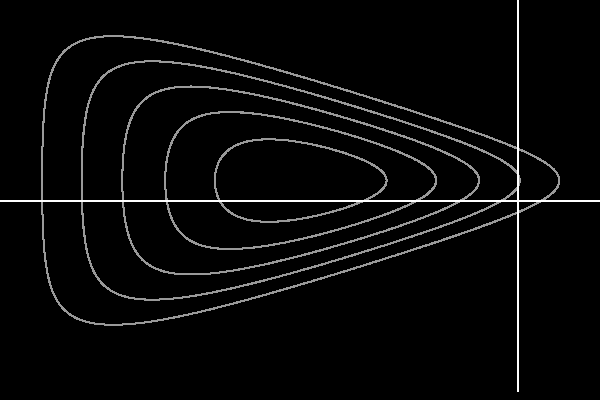
\includegraphics{vis1}\end{center}}
\only<2>{\begin{center}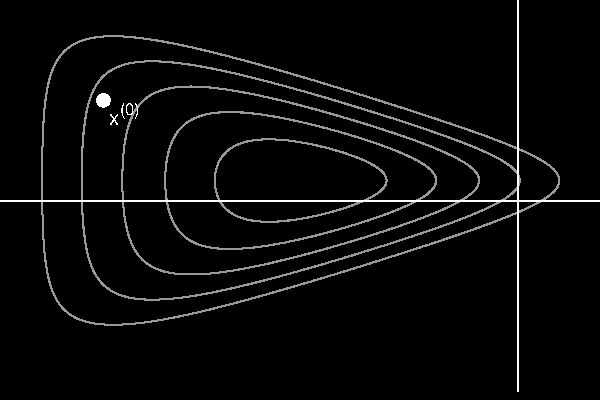
\includegraphics{vis2}\end{center}}
\only<3>{\begin{center}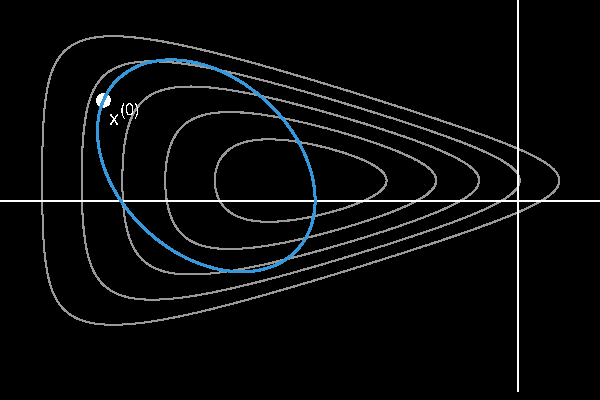
\includegraphics{vis3}\end{center}}
\only<4>{\begin{center}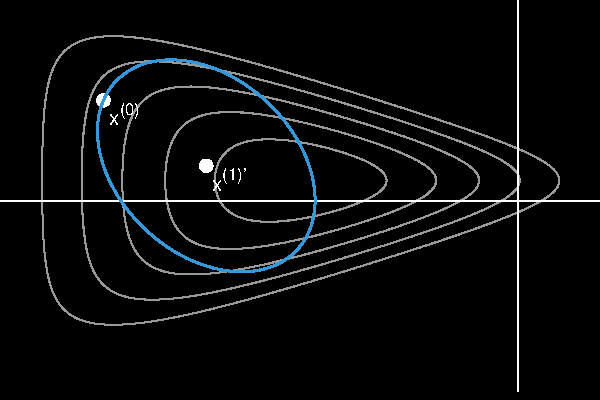
\includegraphics{vis3a}\end{center}}
\only<5>{\begin{center}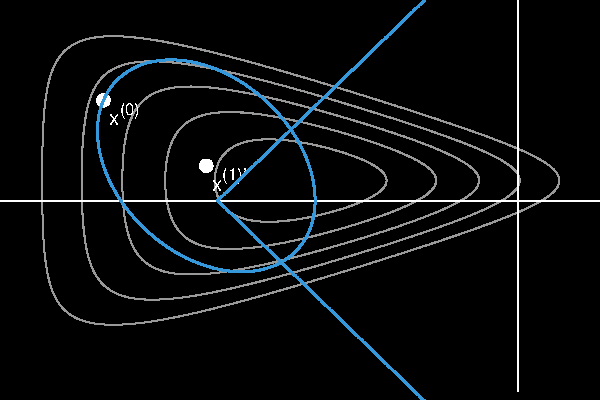
\includegraphics{vis3b}\end{center}}
\only<6>{\begin{center}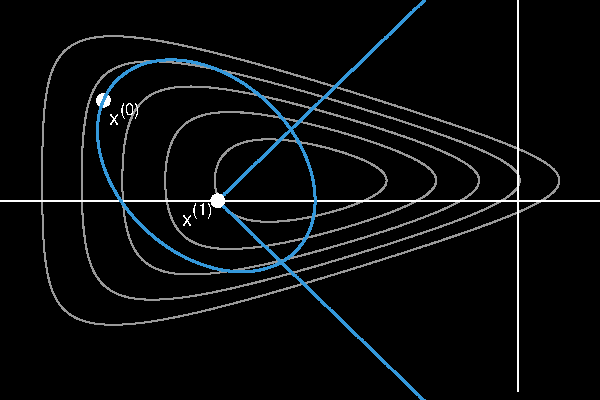
\includegraphics{vis4}\end{center}}
\only<7>{\begin{center}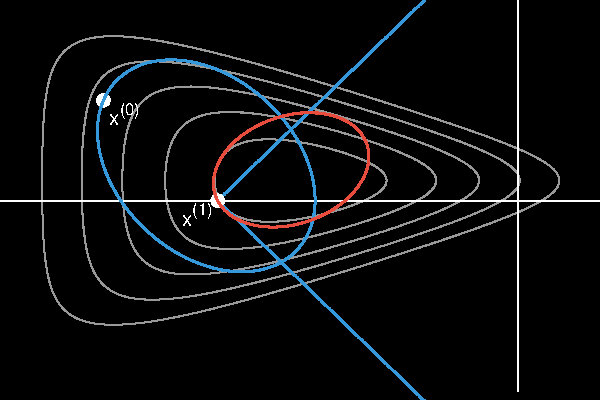
\includegraphics{vis5}\end{center}}
\only<8>{\begin{center}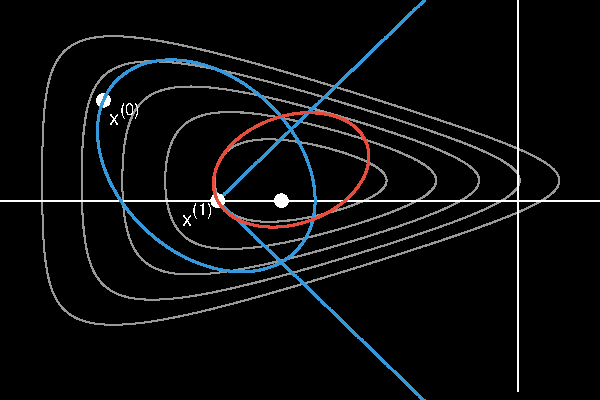
\includegraphics{vis6}\end{center}}
\only<9>{\begin{center}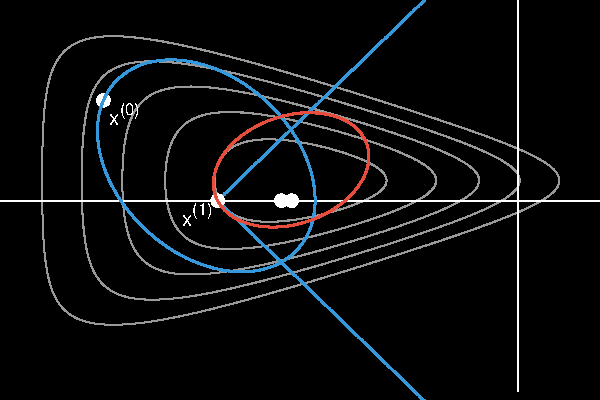
\includegraphics{vis7}\end{center}}
\end{frame}

\begin{frame}
\frametitle{Computational complexity of inner loop}
  \vspace{-0.4in}
  \[
  d = \arg \min_\Delta \hat{f}(x + \Delta) + \lambda\|x + \Delta \|_1
  \] \\
\pause
\vspace{0.3in}
Exploit sparsity using a coordinate descent active set method
\begin{enumerate}
\item Form active set by including coordinate $i$ if
\[
|\nabla f(x)_i| > \lambda \text{ or } x_i \ne 0
\vspace{-2mm}
\]
\item Iteratively minimize, done in closed
  form
\end{enumerate}
\end{frame}

\begin{frame}
\frametitle{Theoretical analysis}
\pause
\begin{center}
It works.
\end{center}
\end{frame}

\begin{frame}
\frametitle{Theoretical analysis (for real)}
\begin{enumerate}
\item The objective $F = f + g$ is nonincreasing, $F > -\infty$
\item $F(x^{k+1}) - F(x^k) \le \sigma \alpha^k\Delta^k \le 0$
\item $\inf_k \alpha^k > 0$
\item $\Delta^k \to 0, d^k \to 0$ as $k \to \infty$
\item $\|x^k  - x^\star\| \to 0$
\end{enumerate}
\end{frame}

\end{document}
